\subsection{Series to Parallel Conversion} \label{subsec:SeriesToParallel}
The $\bar v$ and $\bar i$ signals described in section \refq{sec:ImpedanceAnalysis} can be used to characterize the DUT, but the signals say nothing about how the impedance is supposed to be modelled. The impedance of a DUT could have the form shown on figure \refq{fig:4_1_5_DUTXSeriesParallel} where the DUT has a series resistance $R_s$ in series with a parallel connection of a pure reactance $X$, from either a capacitor or inductor, and a parallel resistor $R_p$. Both $R_s$ and $R_p$ cause power dissipation in the DUT. The value $R_s$ is also known as \textit{equivalent series resistance}, or ESR:

\begin{figure}[H]
    \centering
    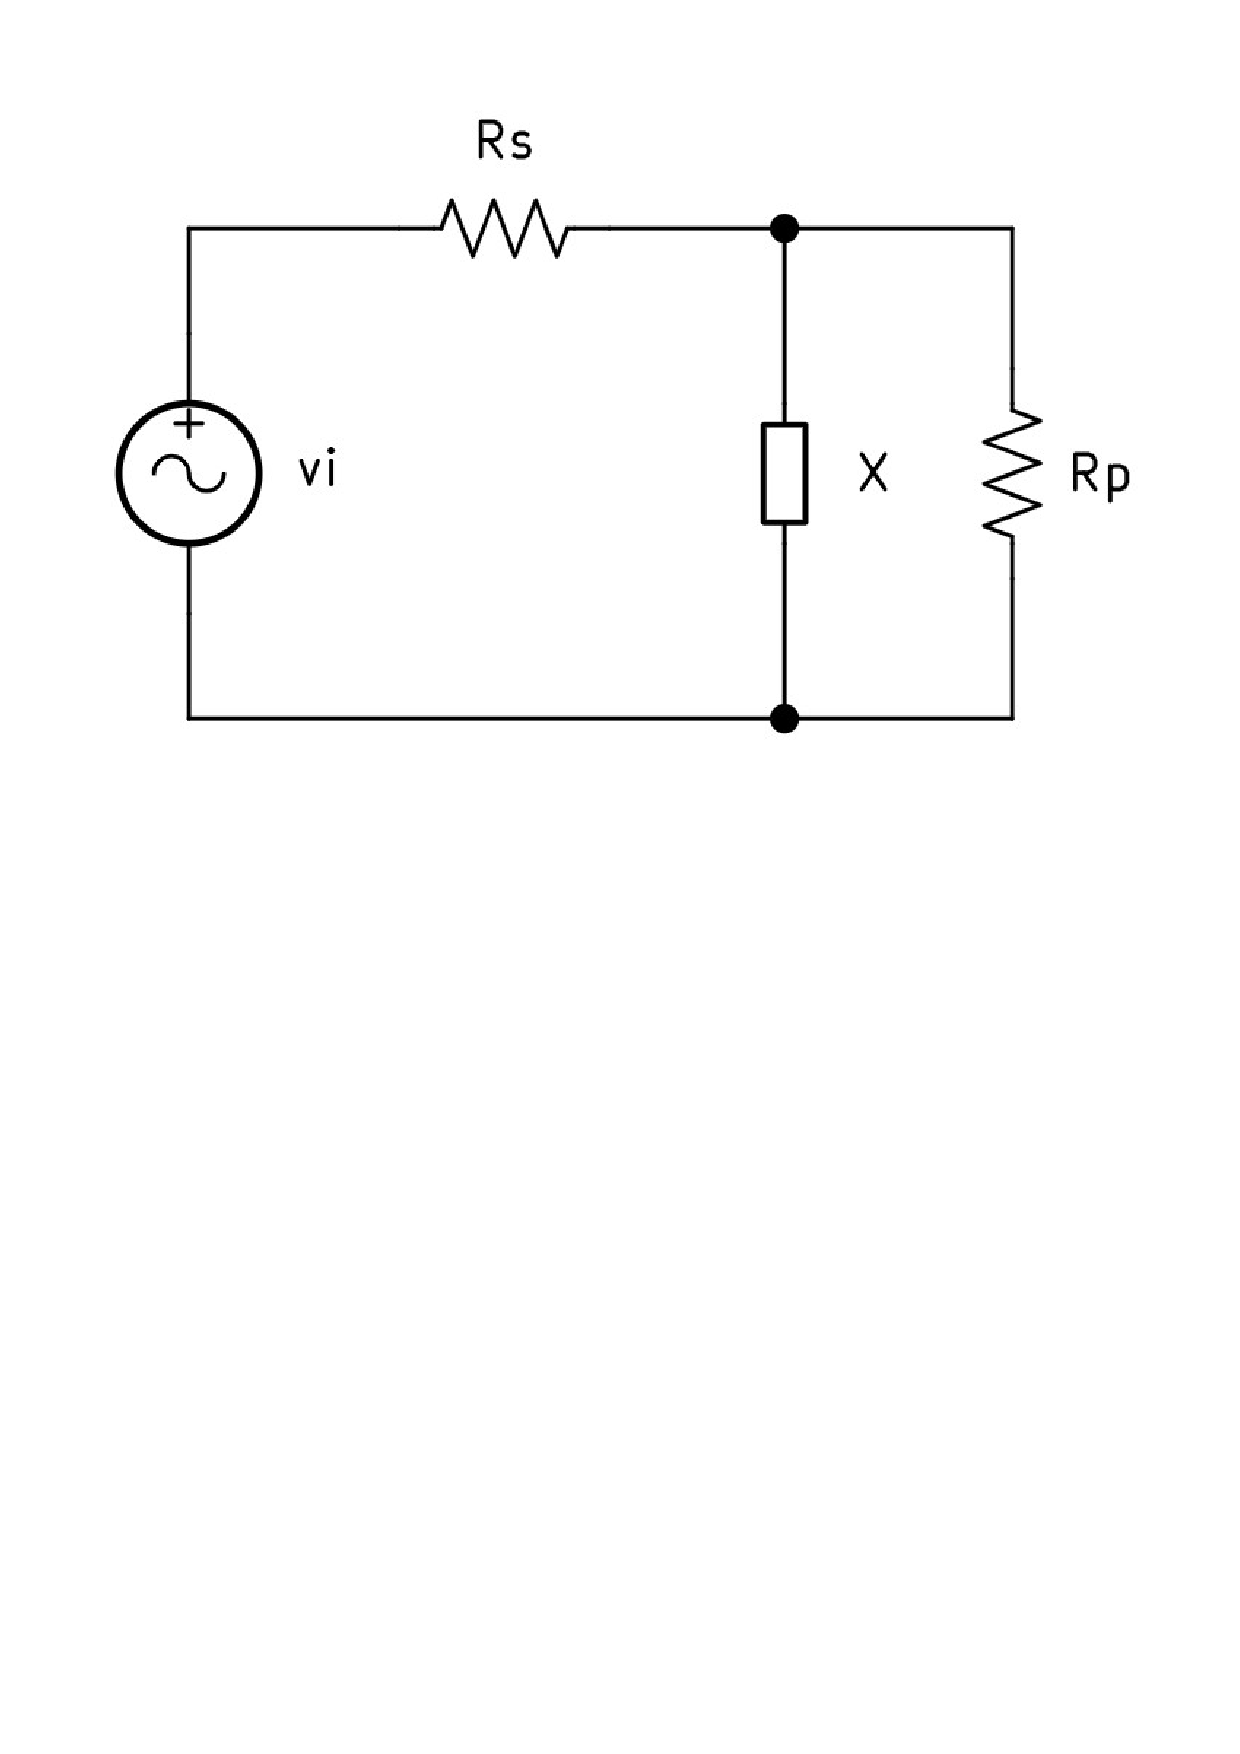
\includegraphics[clip, trim=0 450 0 0, width=0.4\textwidth]{Sections/4_TechnicalAnalysis/Figures/4_1_1_DUTXSeriesParallel.pdf}
    \caption{A simple model of a DUT. The pure reactance X has a series resistance and a parallel resistance.}
    \label{fig:4_1_5_DUTXSeriesParallel}
\end{figure}

If the reactance on figure \refq{fig:4_1_5_DUTXSeriesParallel} is a capacitor then then parallel resistance $R_p$ will, typically, be a large value while the series resistance $R_s$ is small. Eq \refq{eq:4_1_1_CapCurrent5} in section \refq{subsec:Reactance} states that capacitance is inversely proportional to capacitive reactance, so \textit{small} capacitors cause \textit{large} reactance and vice versa. \textit{Small} capacitors are typically used in filter and RF applications where power dissipation in the series resistance is less interesting than the leakage resistance ($R_p$) in the capacitor so it makes sense to model the impedance as a parallel circuit and disregard the series resistance. The series resistance for $large$ filter capacitors in power supply applications will have an impact on the power supplies overall efficiency and the leakage resistance is of less import. In this case it makes sense to model the impedance as a series circuit. The two arrangements that can be used to model the DUT is shown on figure \refq{fig:4_1_5_DUTXSeriesParallelMode}.

\begin{figure}[H]
    \centering
    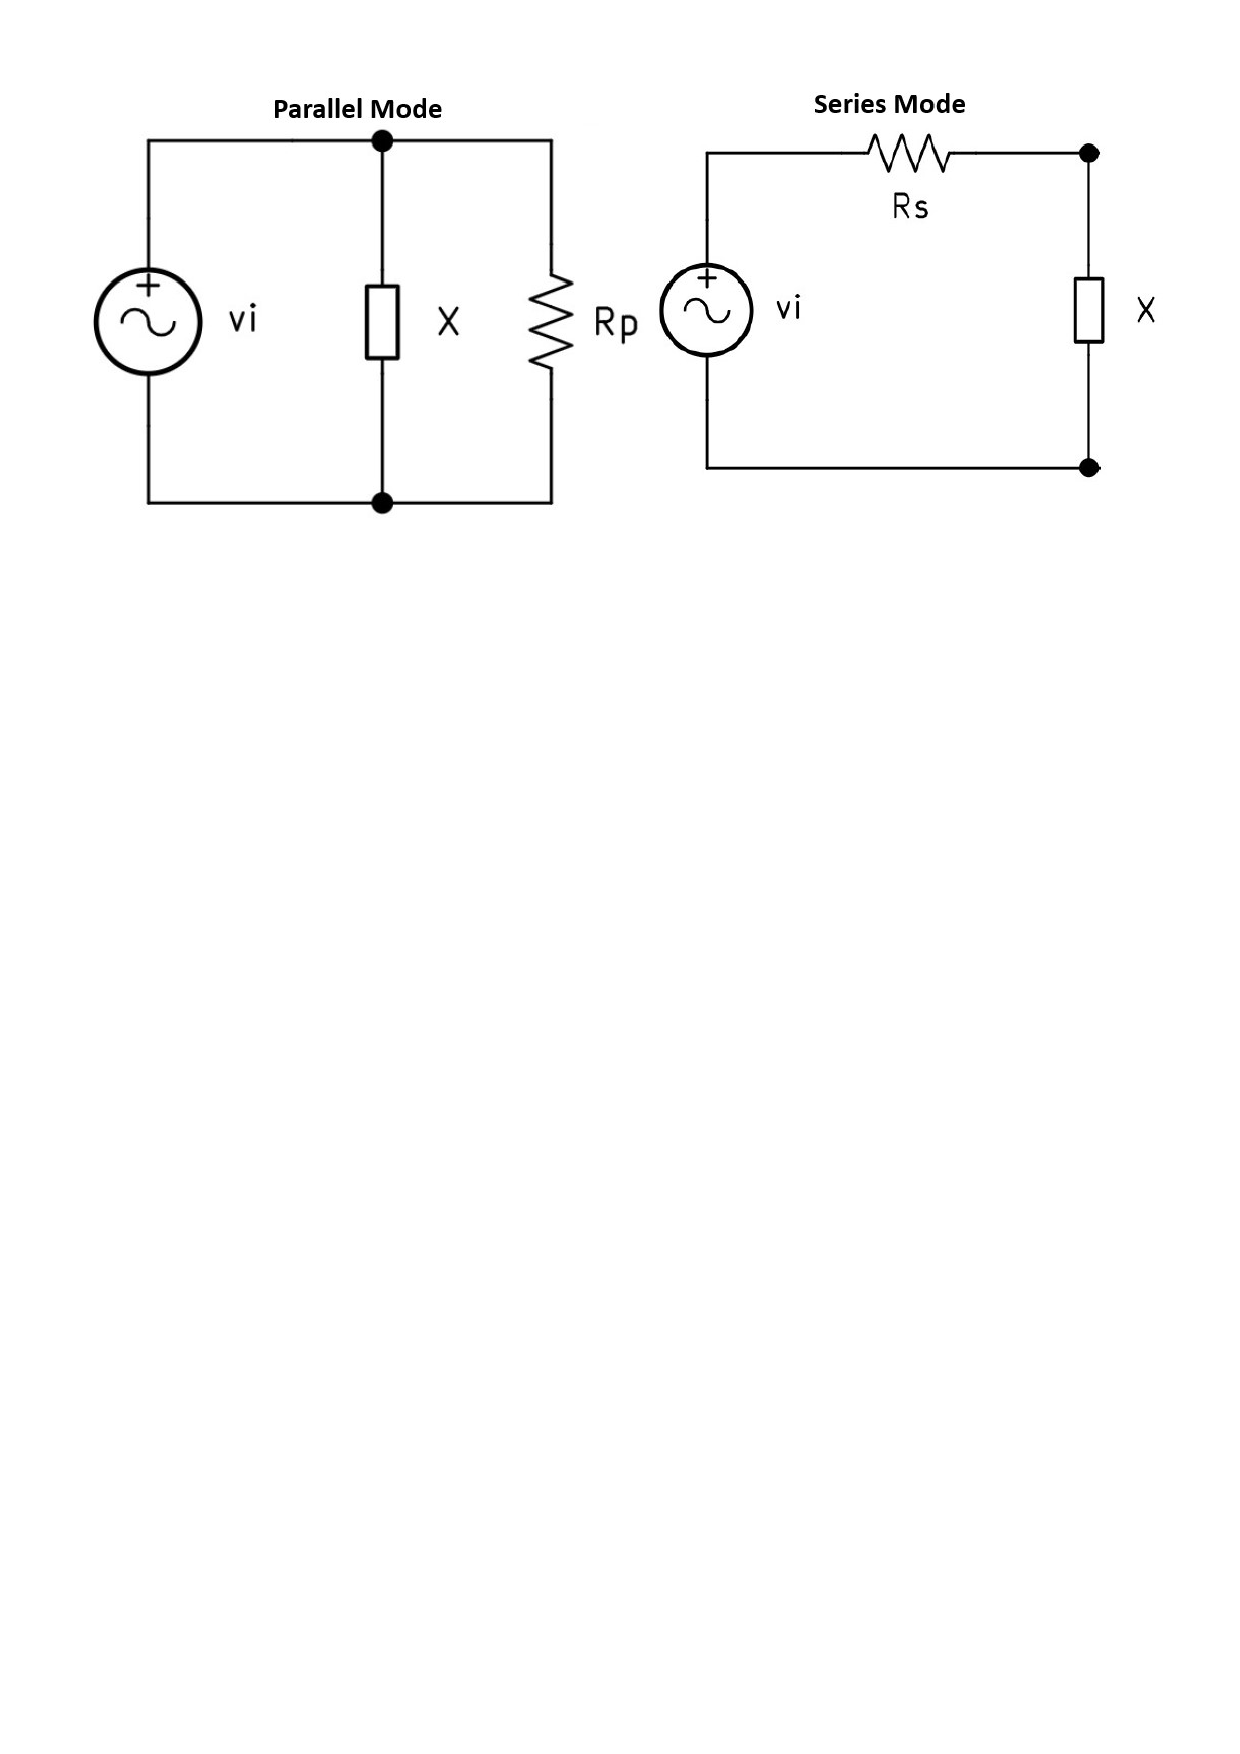
\includegraphics[clip, trim=0 550 0 0, width=0.8\textwidth]{Sections/4_TechnicalAnalysis/Figures/4_1_5_SeriesParallelMode.pdf}
    \caption{The two models that could be used for the DUT. The impedance measured can be fitted to either of them depending on the situation.}
    \label{fig:4_1_5_DUTXSeriesParallelMode}
\end{figure}

Assuming $\bar v$ and $\bar i$ from section \refq{sec:ImpedanceAnalysis} has been measured. The series model can be fitted to the impedance as $\bar Z =|\bar Z| \cdot \mathrm e^{\pm j\phi}$ where Rs and X will be the real and imaginary parts of the complex impedance as shown in eq \refq{eq:4_1_5_SeriesModel1}.

\begin{equation}\label{eq:4_1_5_SeriesModel1}
    \begin{split}
        R_s =& \Re(|\bar Z| \cdot \mathrm e^{\pm j\phi}) = |\bar Z| \cdot cos(\phi)\\
        X =& \Im(|\bar Z| \cdot \mathrm e^{\pm j\phi}) = \pm j\cdot |\bar Z| sin(\phi) 
    \end{split}
\end{equation}

These values in eq \refq{eq:4_1_5_SeriesModel1} can be used to fit the impedance to the series model shown on figure \refq{fig:4_1_5_DUTXSeriesParallelMode}. The admittance of the parallel arrangement can be written as in eq \refq{eq:4_1_5_ParallelModel1}.
\begin{equation}\label{eq:4_1_5_ParallelModel1}
    \bar Y = \frac{|\bar i| [cos(\phi_1) + j\cdot sin(\phi_1)]}{|\bar v| [cos(\phi_0) +j\cdot sin(\phi_0)]}
\end{equation}
Again, like in section \refq{sec:ImpedanceAnalysis}, it is assumed that the reference voltage waveform has $\phi = 0$. This simplifies eq \refq{eq:4_1_5_ParallelModel1} to \refq{eq:4_1_5_ParallelModel2}.
\begin{equation}\label{eq:4_1_5_ParallelModel2}
    \bar Y = \frac{|\bar i| [cos(\phi_1) + j\cdot sin(\phi_1)]}{|\bar v|}
\end{equation}
Simplifying eq \refq{eq:4_1_5_ParallelModel2} and defining that $|\bar Y| = \frac{|\bar i|}{|\bar v|}$to rectangular form gives eq \refq{eq:4_1_5_ParallelModel3}.
\begin{equation}\label{eq:4_1_5_ParallelModel3}
    \bar Y = |\bar Y| cos(\phi_1) + j |\bar Y| sin(\phi_1)
\end{equation}
The real part of the complex admittance is the conductance $G$ while the imaginary part is the susceptance $B$ as shown in eq \refq{eq:4_1_5_ParallelModel4}.
\begin{equation}\label{eq:4_1_5_ParallelModel4}
    \begin{split}
        G =& \Re(|\bar Y| cos(\phi_1) + j |\bar Y| sin(\phi_1)) = |\bar Y| \cdot cos(\phi)\\
        jB =& \Im(|\bar Y| cos(\phi_1) + j |\bar Y| sin(\phi_1)) =  j\cdot |\bar Y| sin(\phi)  
    \end{split}
\end{equation}

The admittance $\bar Y$ can be converted to impedance as shown in eq \refq{eq:4_1_5_ParallelModel4} as impedance is the reciprocal of admittance $Z = \frac{1}{Y}$ as shown in eq \refq{eq:4_1_5_ParallelModel5}.
\begin{equation}\label{eq:4_1_5_ParallelModel5}
    \bar Z = \frac{1}{G + jB} =\frac{G-jB}{G^2 + B^2} = \frac{G}{G^2 + B^2} -j\frac{B}{G^2 + B^2}
\end{equation}
Eq \refq{eq:4_1_5_ParallelModel5} and eq \refq{eq:4_1_5_ParallelModel4} can convert a series impedance into a parallel impendance of the forms show on figure \refq{fig:4_1_5_DUTXSeriesParallelMode}. It is important to note how these models only fit for exactly 1 frequency. They must be recalculated if the test frequency is changed.
